% (C) Marc Lijour, 2019 
% Licensed under a Creative Commons License BY-SA
% https://creativecommons.org/licenses/by-sa/2.5/ca/
% Presentation for the Blockchain Developer Certificate students at George Brown College
% Hands-on Introduction to Blockchain
% 
% Variables
% TODO set the variables
% ---------------------- USER-DEFINED --------------------------------
\newcommand{\CEtitle}{Blockchain~Developer~Certificate}
\newcommand{\CElongtitle}{Blockchain and Loyalty programs}
\newcommand{\CEsubtitle}{for George Brown College students}
\newcommand{\CEauthor}{Marc~Lijour}
\newcommand{\CEdate}{November~6, 2019}
\newcommand{\CEsubject}{GBC~Blockchain}
% --------------------------------------------------------------------
% Template
% (C) Marc Lijour, 2019
% This document is licensed under a Creative Commons License BY-SA (feel free to use the code, but all rights are reserved for logos and art)
% https://creativecommons.org/licenses/by-sa/2.5/ca/
% Creative Emergy (CE) presentation template in LaTeX
% This template comes with a first page on a picture background
% Possible improvement in future iterations
% - Test and fix as needed to work on xetex (to use Ubuntu fonts)
% === USAGE===
% Create a file for your LaTeX content (slides, etc), in which you must do the following:
% TODO 1 - set variables defined below
% TODO 2 - include this code by calling: \input{<the name of this document>}
% TODO 3 - Start the document as usual and you're in business; just use \begin{document} and don't forget to conclude with \end{document}
% TODO 4 - Use the custom method \CEcoverpage instead of \titlepage to create your cover page
% Voilà!
%
\documentclass[utf8]{beamer}
\usepackage{etoolbox}
%\usepackage[american,french]{babel}
%\usepackage[T1]{fontenc}
%\usepackage[utf8]{inputenc}
% Variables
% ---------------------- USER-DEFINED --------------------------------
\ifdef{\CEtitle}{}{\newcommand{\CEtitle}{\color{red}Title TBD}}
\ifdef{\CElongtitle}{}{\newcommand{\CElongtitle}{\color{red}Long title TBD}}
\ifdef{\CEsubtitle}{}{\newcommand{\CEsubtitle}{\color{red}Subtitle TBD}}
\ifdef{\CEauthor}{}{\newcommand{\CEauthor}{\color{red}Author TBD}}
\ifdef{\CEdate}{}{\newcommand{\CEdate}{\color{red}Date TBD}}
\ifdef{\CEsubject}{}{\newcommand{\CEsubject}{\color{red}Subject TBD}}
% --------------------------------------------------------------------
\usetheme{Boadilla}
% Set color close to CE paletter
%\definecolor{beamer@blendedblue}{RGB}{150,36,36}
\definecolor{beamer@blendedblue}{RGB}{124,42,39}
% Cover Page
\title[\CEtitle] {\CElongtitle}
\subtitle{\CEsubtitle}
\author{\CEauthor}
\date{\CEdate}
\subject{\CEsubject}
\usepackage{tikz}
% Try Xetex to use system fonts (pdflatex makes it hard to import a font)
%\usepackage{fontspec}
%\setsansfont{Ubuntu}
%\setmonofont{Ubuntu Mono}

% -- create a custom (command) title page -which has the benefit of not affecting the settings for the rest of the presentation
\newcommand{\CEcoverpage}{\frame[plain]{
	\tikz[remember picture,overlay] {
        	\node(bkgd) at ([xshift=0cm,yshift=0cm]current page.center) 
			{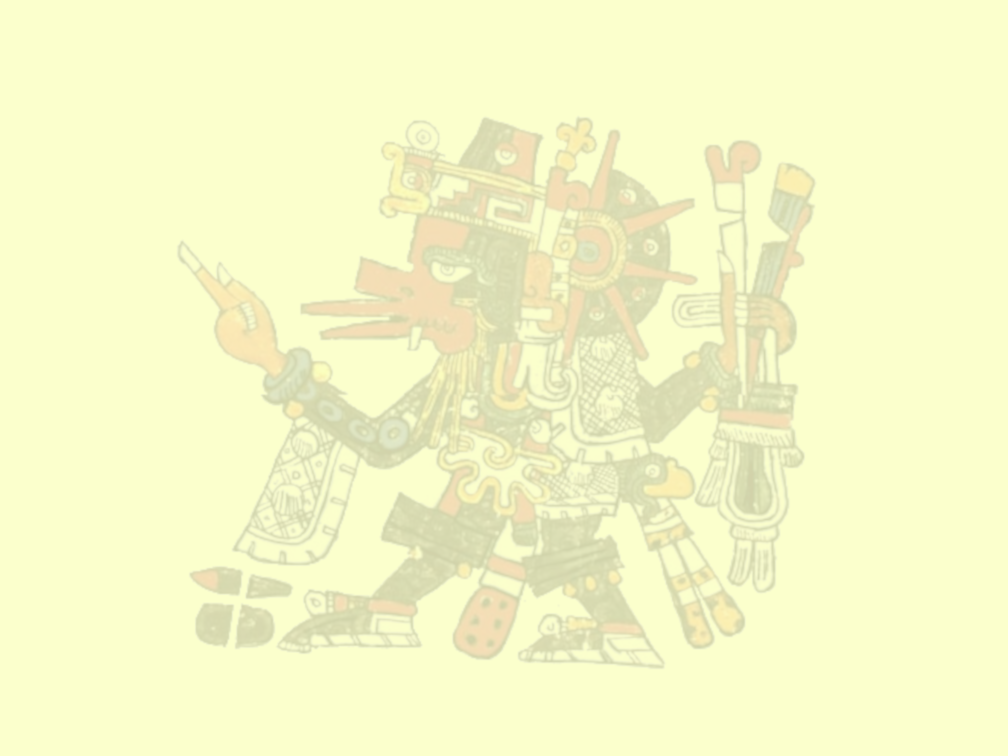
\includegraphics[width=\paperwidth, height=\paperheight]{../../Creative_Emergy-LaTeX_Templates/images/bkg3}};
        	\node(logo) at ([xshift=-4.2cm,yshift=3.5cm]current page.center) 
		 	{
\includegraphics[scale=.1]{../../Creative_Emergy-LaTeX_Templates/images/ce_logo_hr_name}};
        	\node(CC-BY-SA) at ([xshift=5cm,yshift=-4cm]current page.center) 
			{\href{https://creativecommons.org/licenses/by-sa/2.5/ca/}{
\includegraphics[scale=.4]{../../Creative_Emergy-LaTeX_Templates/images/CC-BY-SA-403x141}}};
	}
	\tikz[remember picture,overlay] {
        	\node(title) at ([xshift=0cm,yshift=0cm]current page.center) 
			%{\Large\color{black}\textbf{{\CElongtitle}}};
			{\Large\color{beamer@blendedblue}\textbf{{\CElongtitle}}};
        	\node(subtitle) at ([xshift=0cm,yshift=-.7cm]current page.center) 
			{\small\color{beamer@blendedblue}\emph{\CEsubtitle}};
        	\node(author) at ([xshift=0cm,yshift=-2cm]current page.center) 
			{\small\color{beamer@blendedblue}By~\CEauthor};
        	\node(date) at ([xshift=0cm,yshift=-2.5cm]current page.center) 
			{\tiny\color{beamer@blendedblue}\CEdate};
        	\node(footnote) at ([xshift=0cm,yshift=-3.9cm]current page.center) 
			{\TINY\color{beamer@blendedblue}\emph{The Art and Science of Eternal Blossom}};
        	%\node(footnote) at ([xshift=0cm,yshift=-4.1cm]current page.center) 
		%	{\TINY\color{black}\emph{focusing on Blockchain and related technologies}};
    	}
}}
%
% This sets the ColliderX logo at the bottom right corner of each page
\logo{
	
\includegraphics[scale=.07]{../../Creative_Emergy-LaTeX_Templates/images/Quetzalcoatl_Ourobouros-coloured-same}
}
\AtBeginSection[]
{
  \begin{frame}
    \frametitle{Table of Contents}
    \tableofcontents[currentsection]
  \end{frame}
}
%\usepackage{newunicodechar}
%\usepackage[format=plain,justification=raggedright,singlelinecheck=false]{caption}
\usepackage[format=plain,justification=justified,singlelinecheck=false]{caption} % use this in document to remove "figure": 
%	\captionsetup{labelformat=empty}\caption{caption content} 
% or
% 	\caption*{caption content here}
\usepackage{dirtytalk}
\usepackage{wrapfig}
\usepackage{hyperref}
\usepackage{verbatim}
\usepackage{mathabx}
%\usepackage{MnSymbol}
\usepackage{fancyvrb}


% Extra packages
\usepackage{amssymb}
\usepackage{amsmath}
\usepackage[american]{babel}
\usepackage{csquotes}
\usepackage[backend=biber,style=apa]{biblatex}
\DeclareLanguageMapping{american}{american-apa}
% Use one bib file per section
\addbibresource{references.bib}
\addbibresource{references-loyalty.bib}
\definecolor{links}{HTML}{2A1B81}
\hypersetup{colorlinks,linkcolor=,urlcolor=links}
\usepackage[justification=centering]{caption}
\AtBeginBibliography{\footnotesize}
% Start of the document
\begin{document}
% Cover page
% Do not use this: \frame{\titlepage}
% use this instead:
\CEcoverpage

% Content
% (C) Marc Lijour, 2019 
% Licensed under a Creative Commons License BY-SA
% https://creativecommons.org/licenses/by-sa/2.5/ca/
% Presentation for the Blockchain Developer Certificate students at George Brown College
% ICOs and elements of a white paper

\frame{ 
	\frametitle{The good features of a Blockchain}
    \begin{itemize}
        \item Trust
        \item Transparency
        \item Tamper-resistant
        \item Third-parties involved: Consensus
        \item Transfer of money/valuable commodities
        \item Tied to identity and yet capable of preserving privacy and anonymity
        \item Treasures ownership at the edge (decentralized)
    \end{itemize}
}

% ======================================================================================================
%                         Loyalty Programs 
% ======================================================================================================
% - status today (before blockchain)

\section{Loyalty programs}

\frame{
    \frametitle{Loyalty programs}
    \begin{block}{Definition}
       Loyalty programs are marketing devices to ensure a greater degree of repeat business.
    \end{block}

    \begin{exampleblock}{Examples}
        Frequent flyer miles (e.g. Aeroplan), points cards (e.g. Air miles, Optimum), rewards for credit cards, coffee, hotels, car rentals\ldots
    \end{exampleblock}
}

\frame{
	\frametitle{Market size}
	\begin{figure}
        \centering
		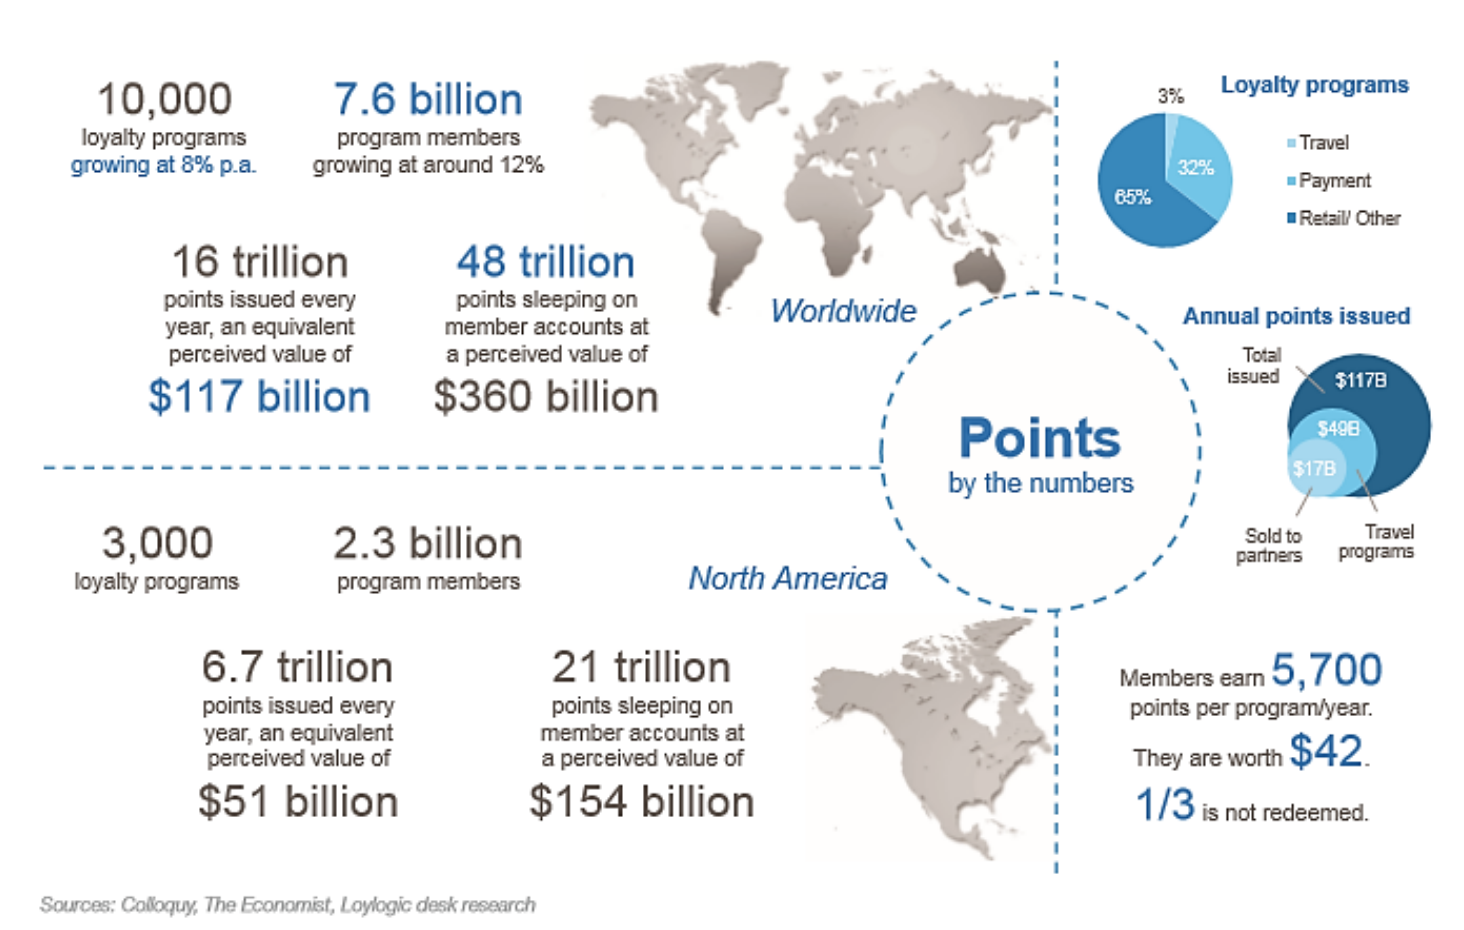
\includegraphics[width=11cm]{../pics/loyalty/colloquy-stats}
        \caption{Colloquy numbers cited in \cite{tokenasia2019:loyalty}}
	\end{figure}
}

\frame{
    \frametitle{How it works}
    \framesubtitle{The customer acquires points}
    \begin{itemize}
        \item get a welcome bonus amount of points
        \item buy a service online or through an app to accumulate points
        \item swap a card in-store
        \item in some other forms, a subscription and level service such as Costco or Amazon prime (the more you pay, the better the deal)
    \end{itemize}
}

\frame{
    \frametitle{How it works}
    \framesubtitle{The customer redeems points}
    \begin{itemize}
        \item customer goes to a website to exchange points for a concrete reward of their choice
        \item customer exchange points for a discount pool (e.g. ESSO)
        \item customer can forfeit points in-store for a service (e.g. a "free" bottle of water, a "free" car wash)
        \item sometimes a free coffee (birthday or every x purchases)
    \end{itemize}
}

\frame{
	\frametitle{What really happens}
	\begin{figure}
        \centering
		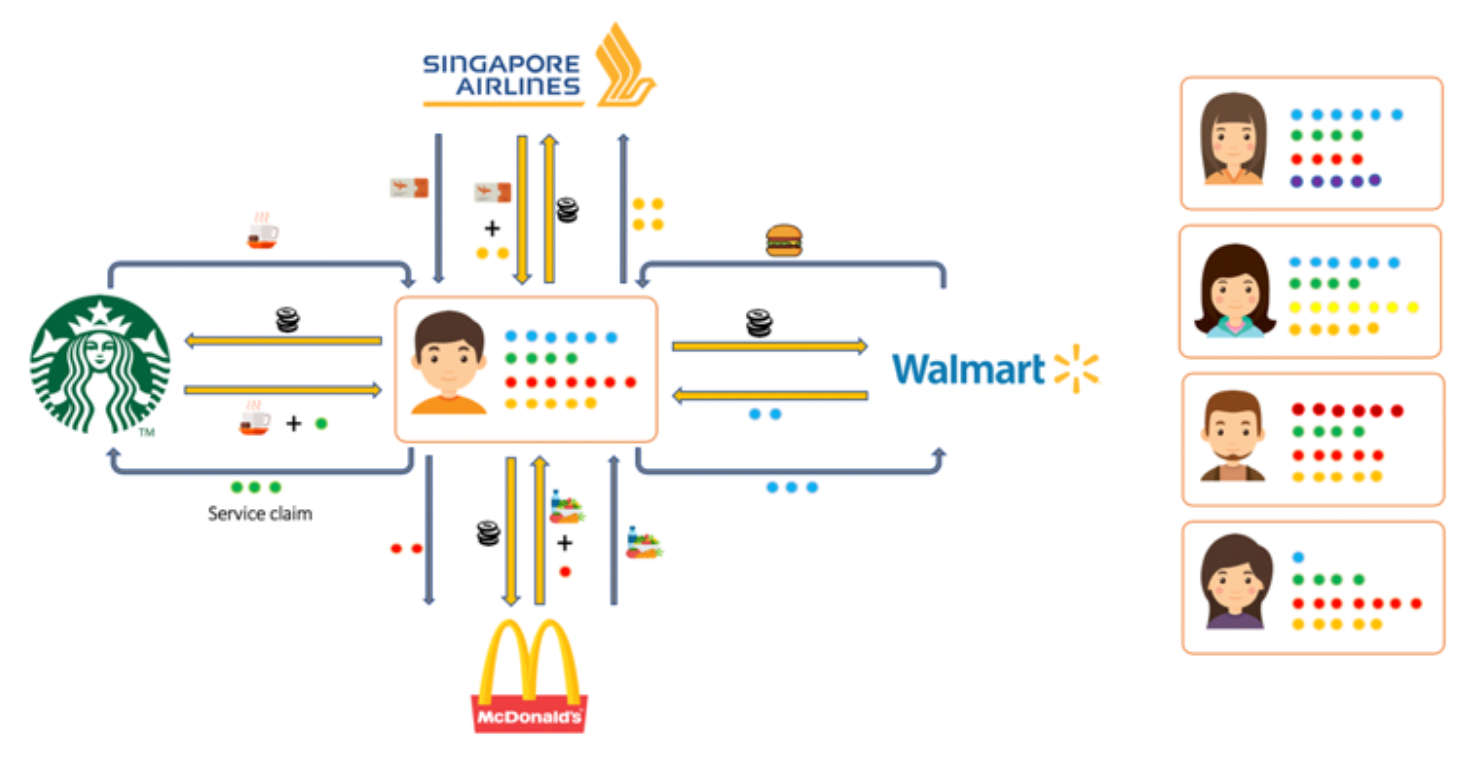
\includegraphics[width=11.5cm]{../pics/loyalty/tomochain-loyalty-complex}
        \caption{\cite{tomochain2019:loyalty}}
	\end{figure}
}


\frame{
    \frametitle{Problem}
    \begin{itemize}
        \item it's a hassle to redeem (go online, etc)
        \item there is no easy connection with partner loyalty programs that would facilitate the exchange of points
        \item the programs can be expensive to administer (especially when not digitized)
        \item programs can go away (e.g. Aeroplan)
        \item dubious economic deal for the customer considering net present value and limited options to cash out
    \end{itemize}
    As a result, most people don't redeem their points\ldots \\
    % the 2016 Bond loyalty report finds that only 50% are active users, and only 20% of those actually redeem their rewards
    \vspace{1em}
    However, enrollment in loyalty programs across various industries in the US grew by 20 percent to 3.32 billion in
2015, and 80 to 90\% or people are more likely to choose a bank that offered rewards, according to \citeauthor{deloitte2016:blockchain:loyalty} (\citeyear{deloitte2016:blockchain:loyalty}).
}

% ======================================================================================================
%                         Blockchain Solutions 
% ======================================================================================================
% - what blockchain brings to the picture
% - notable illustrations and examples

\section{Blockchain solutions}


\frame{
    \frametitle{A better way to run loyalty programs}
%    \cite{deloitte2016:blockchain:loyalty}
    Improvements such as
    \begin{itemize}
        \item interconnection between several programs
        \item full digitization capabilities, including payments
        \item possibility for secondary markets
    \end{itemize}
    Lead to
    \begin{block}{a happier customer}
        \begin{itemize}
            \item more choice to redeem points
            \item faster, almost instantaneous "can pay with points" experience, in-store or online
            \item better deals in secondary markets 
            \item possibility to gift points to family and friends
        \end{itemize}
    \end{block}
    (and more cost-efficient programs at the same time)
}

\frame{
	\frametitle{An example from the \citeauthor{deloitte2016:blockchain:loyalty} paper}
	\begin{figure}
		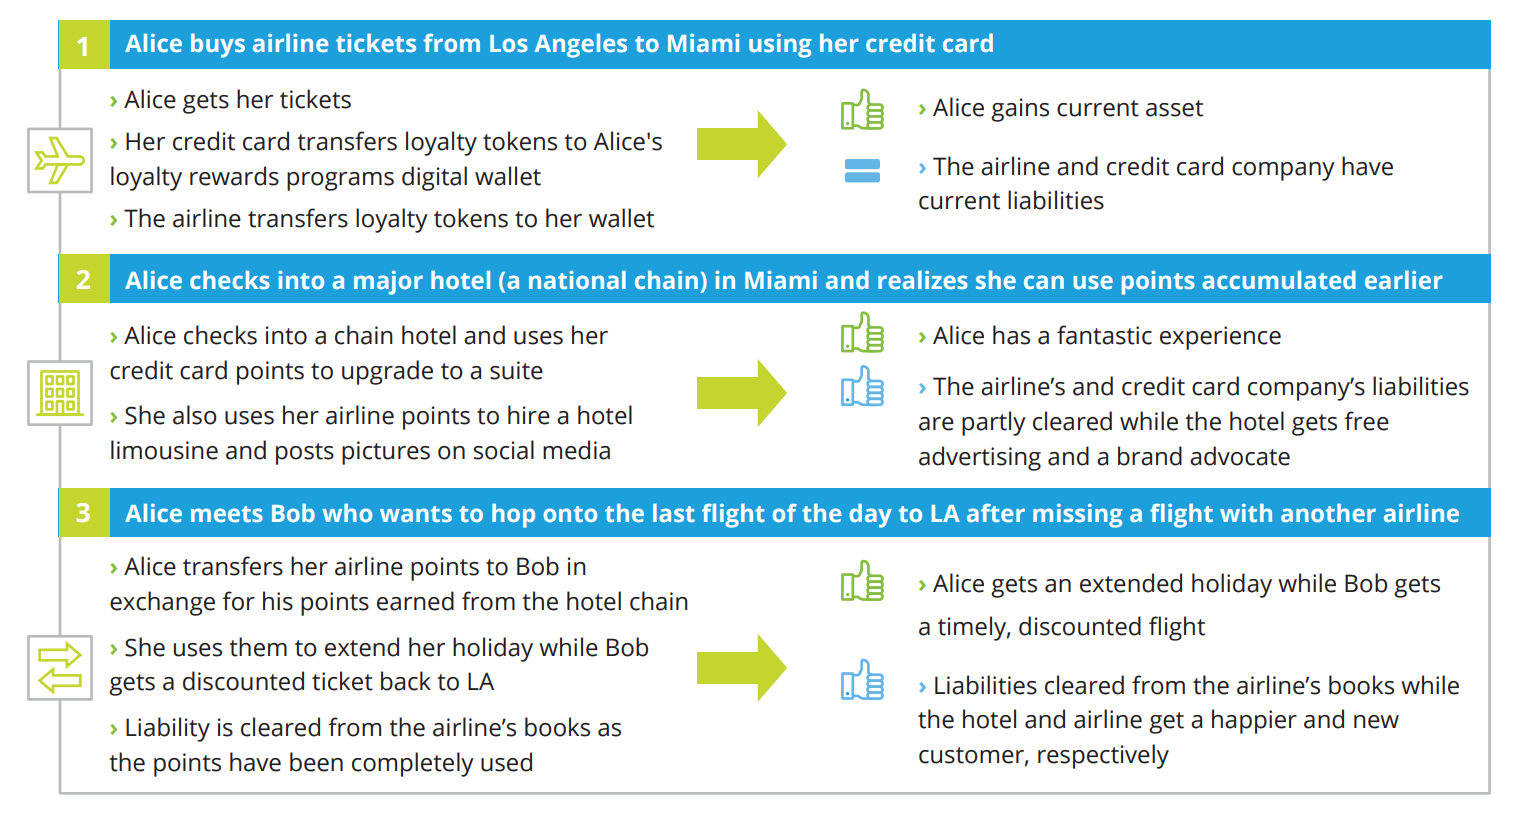
\includegraphics[width=11.5cm]{../pics/loyalty/deloitte-loyalty-customer-journey}
	\end{figure}
}

\frame{
    \frametitle{A smart token}
    \begin{block}{Extra token features}
    vesting schedule to unlock capabilities, space and time constraints, varying degrees of uniqueness (scarcity can command higher value for those items)
    \end{block}    
}

\frame{
    \frametitle{User control}
    \begin{exampleblock}{Features}
    The user collects the points on his/her own wallets (vs. logging to multiple websites).\\
    \vspace{1em}
    \textbf{Privacy}: the merchant can technically accept points as value on the sole basis of the token, without the need to verify the identity of the customer, by trusting the verification has been made earlier.\\
    \vspace{1em}
    \textbf{Transparency} and \textbf{persistence}: the rules are committed on the blockchain for everyone to read (in a tamper-resistant way). The points remain tradeable even after the issuer (possibly) goes out of business.
    \end{exampleblock}
}

% ======================================================================================================
%                         Illustrations 
% ======================================================================================================
% 

\section{Illustrations}

\frame{
	\frametitle{American Express}
	\begin{figure}
        \centering
		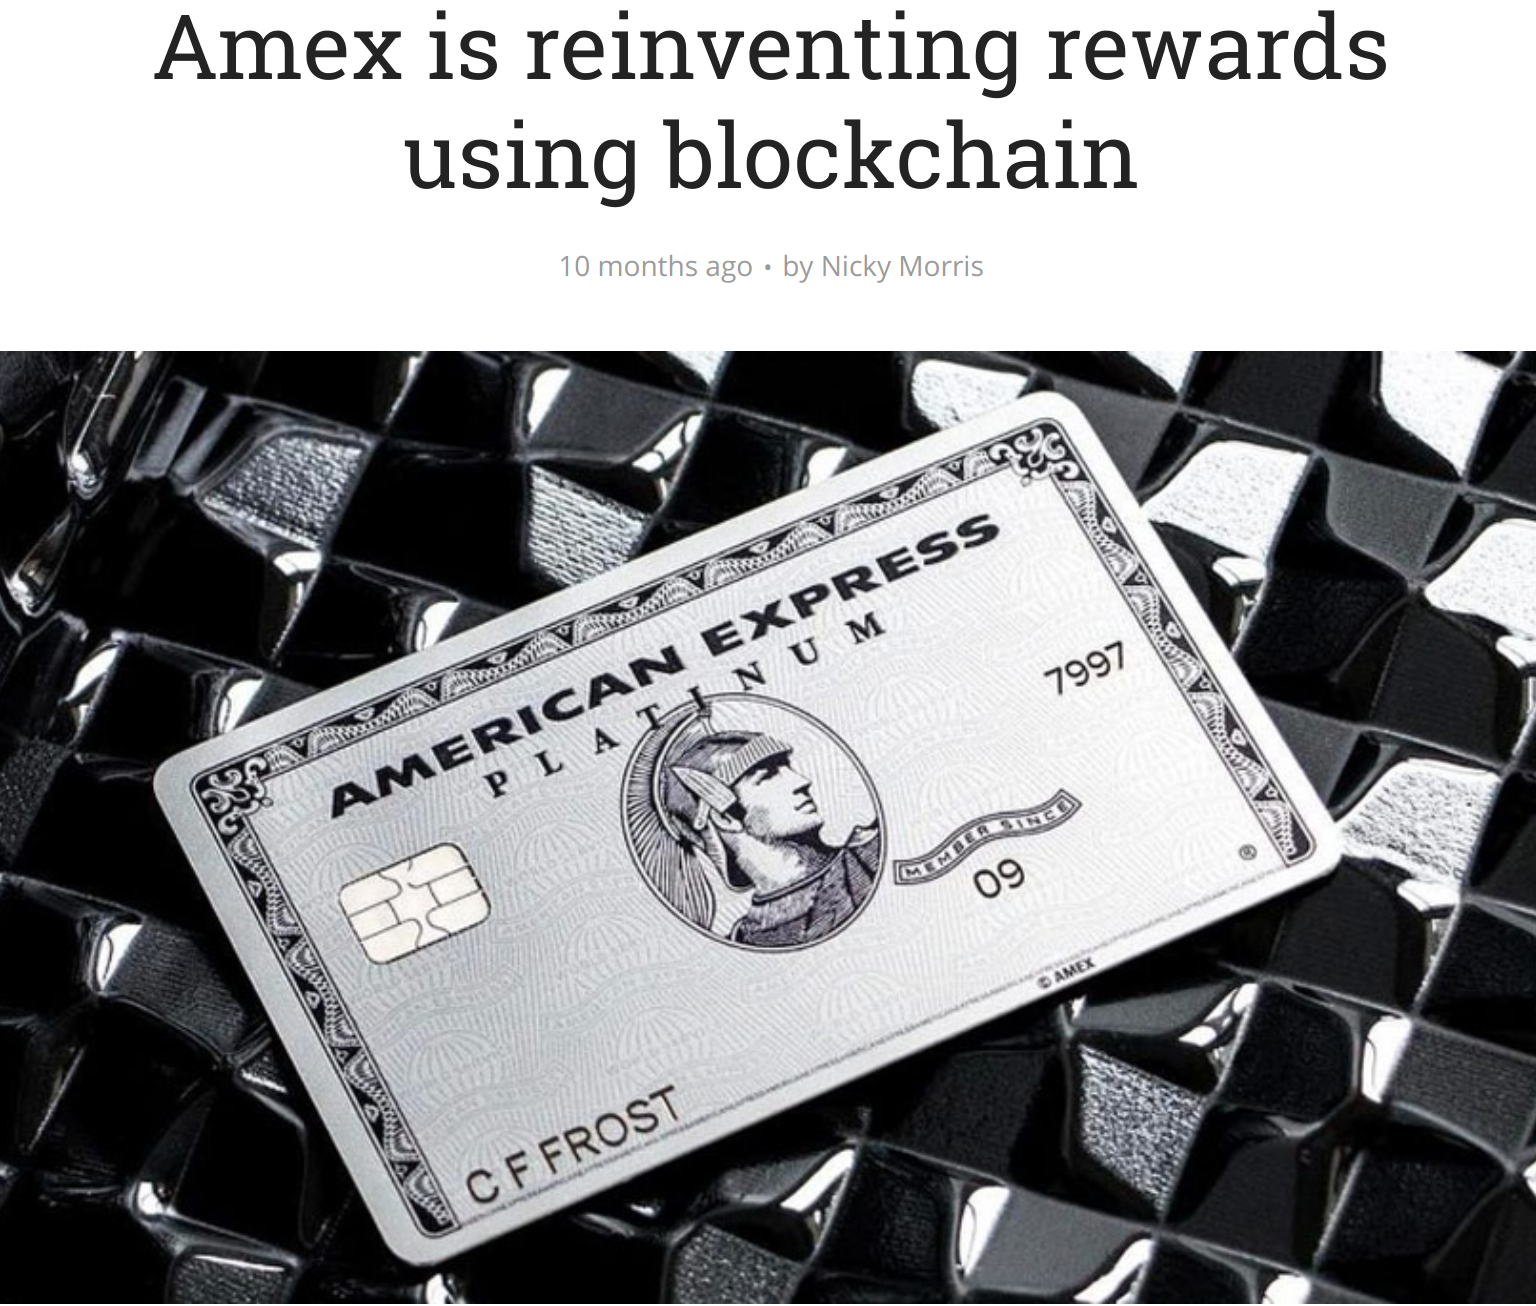
\includegraphics[height=6.5cm]{../pics/loyalty/amex-loyalty}
        \caption{\url{https://www.ledgerinsights.com/amex-blockchain-rewards-american-express/}}
	\end{figure}
}

\frame{
	\frametitle{Bunz}
	\begin{figure}
        \centering
		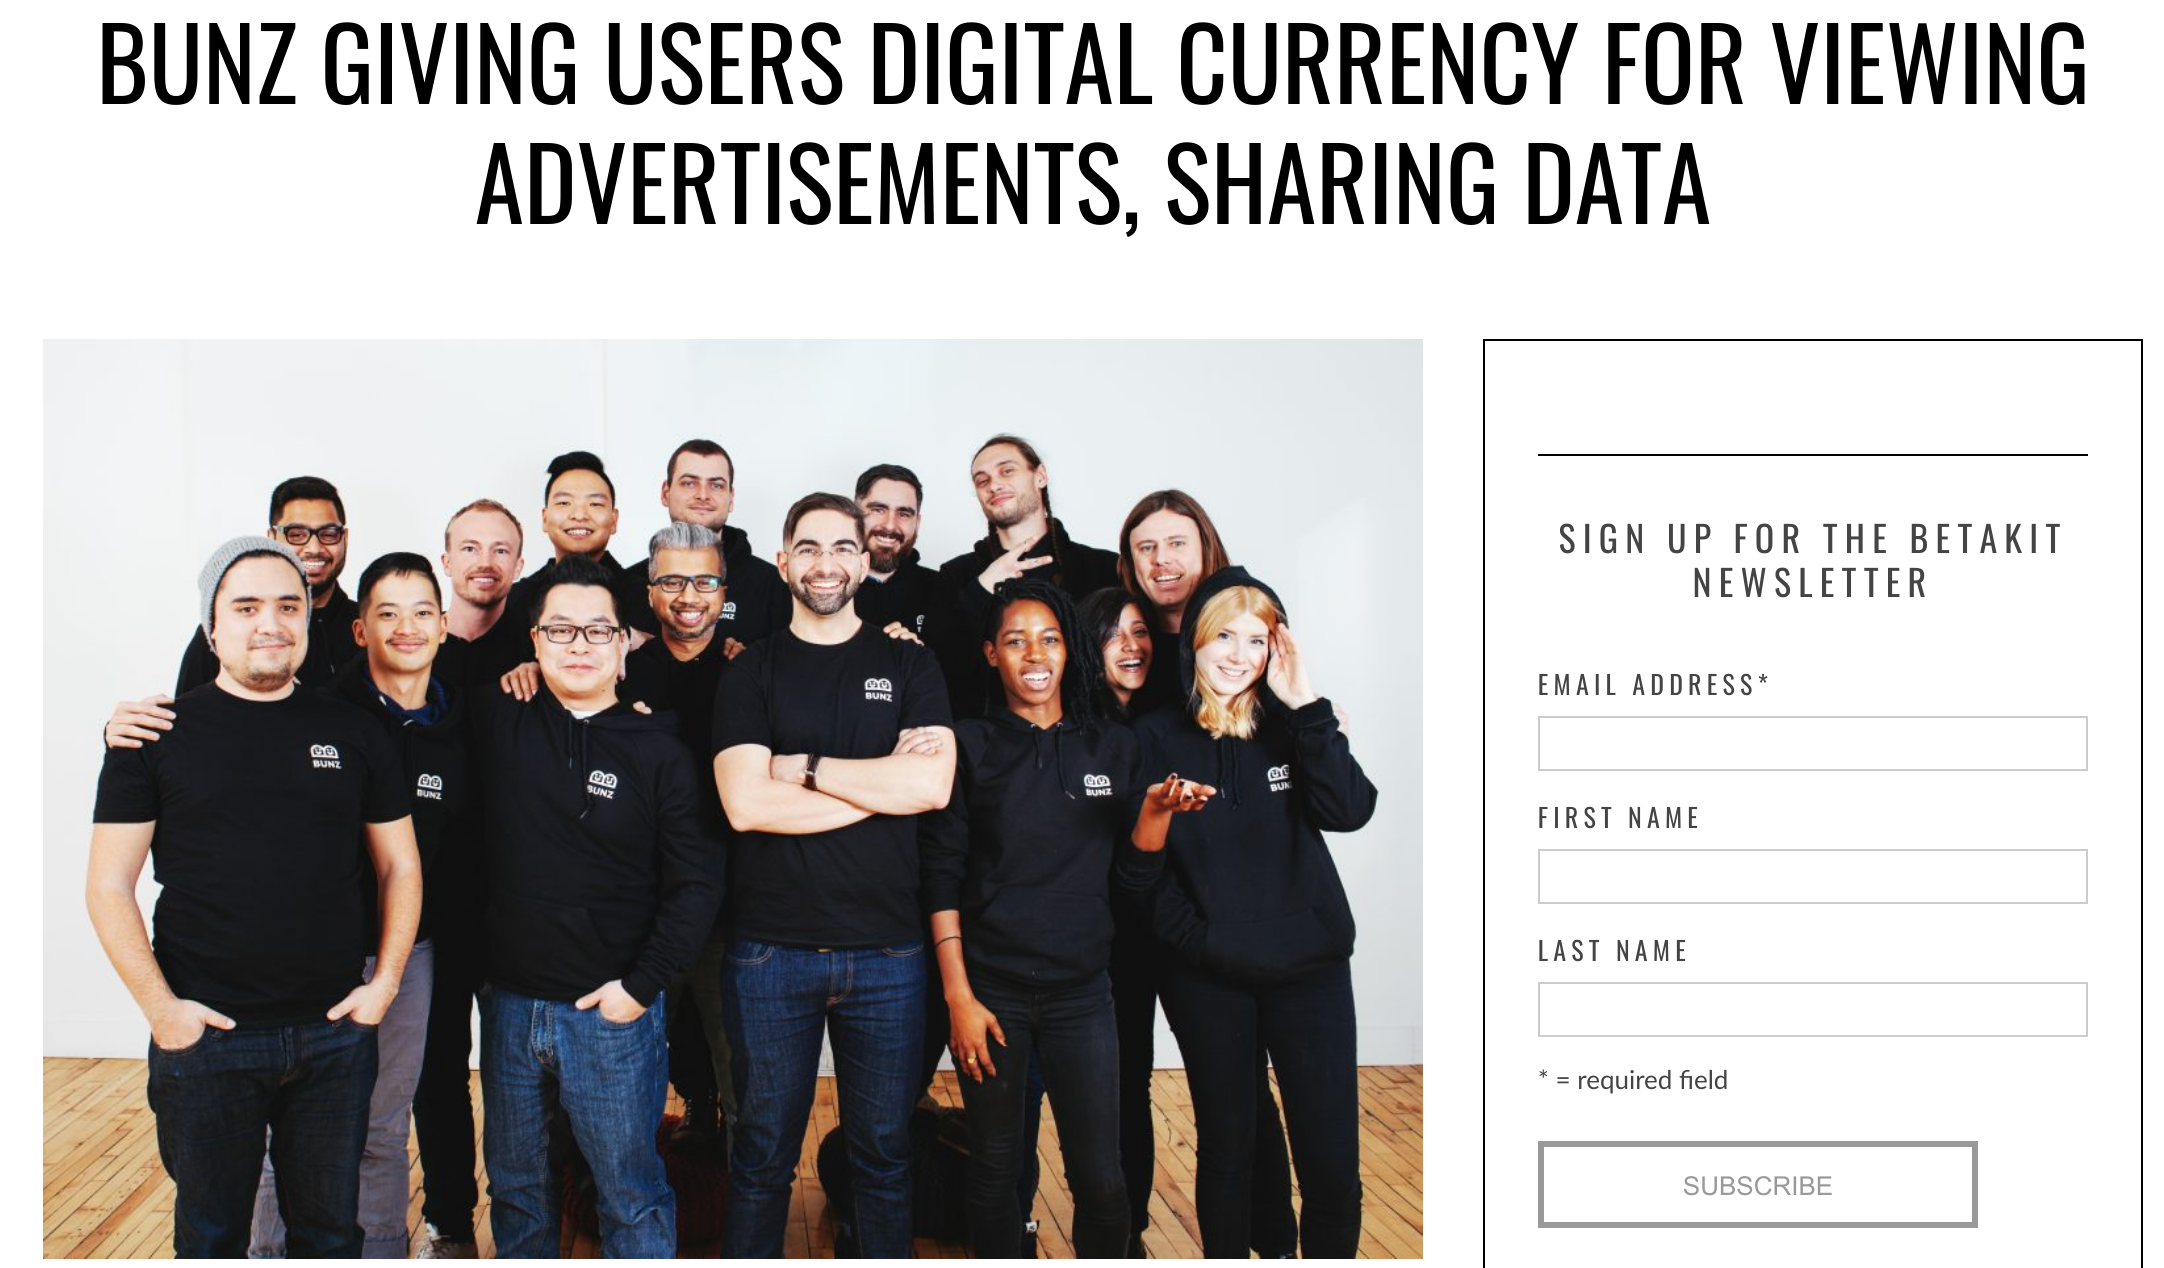
\includegraphics[width=11.5cm]{../pics/loyalty/betakit-bunz}
        \caption{\url{https://betakit.com/bunz-giving-users-digital-currency-for-viewing-advertisements-sharing-data/}}
	\end{figure}
}

\frame{
	\frametitle{qiibee}
	\begin{figure}
        \centering
		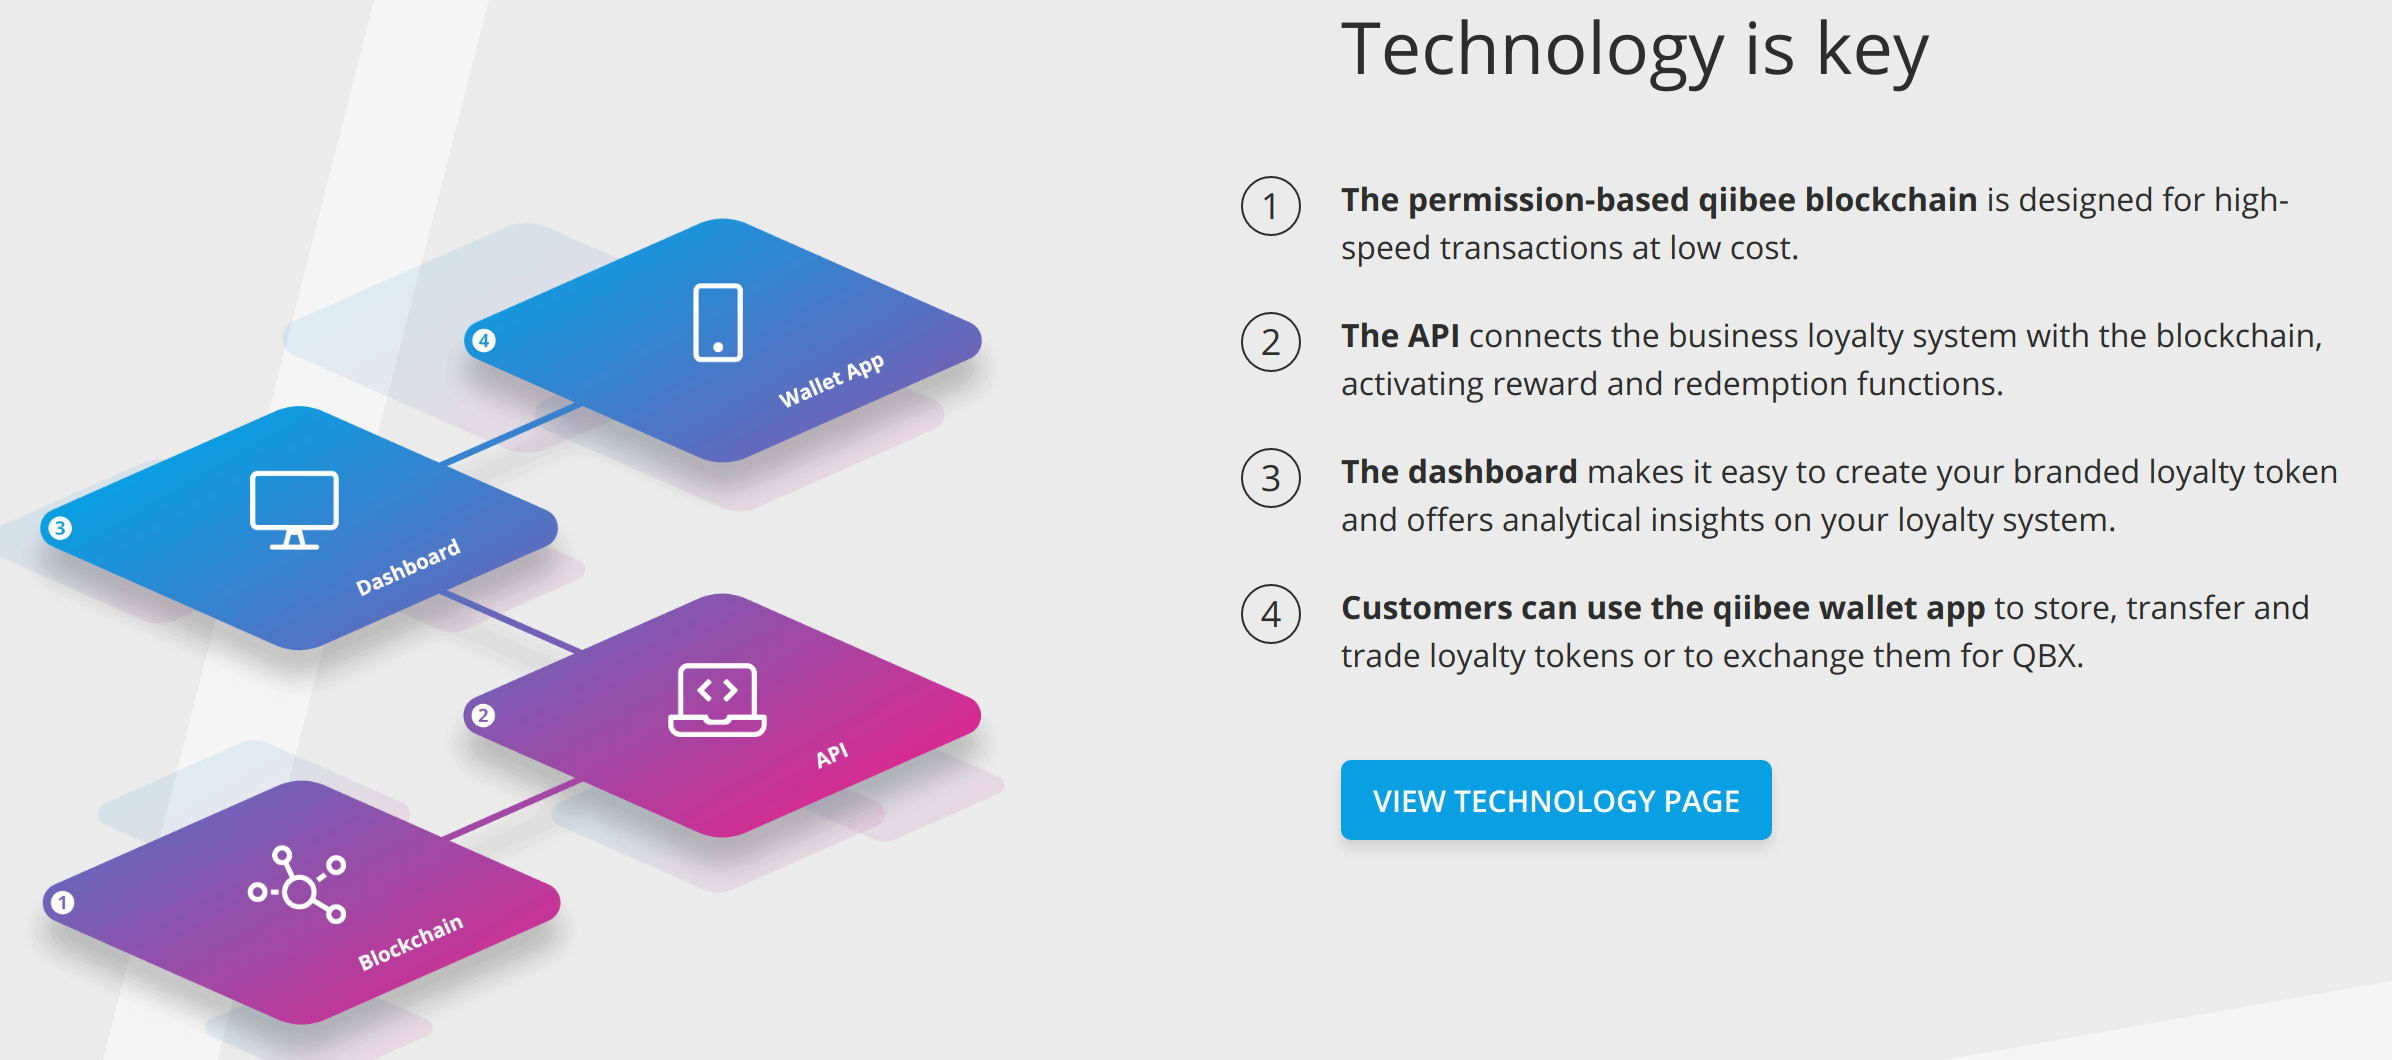
\includegraphics[width=11.5cm]{../pics/loyalty/qiibee}
        \caption{\url{https://qiibee.com/technology}}
	\end{figure}
}


\frame{
	\frametitle{LoyaltyOne}
	\begin{figure}
        \centering
		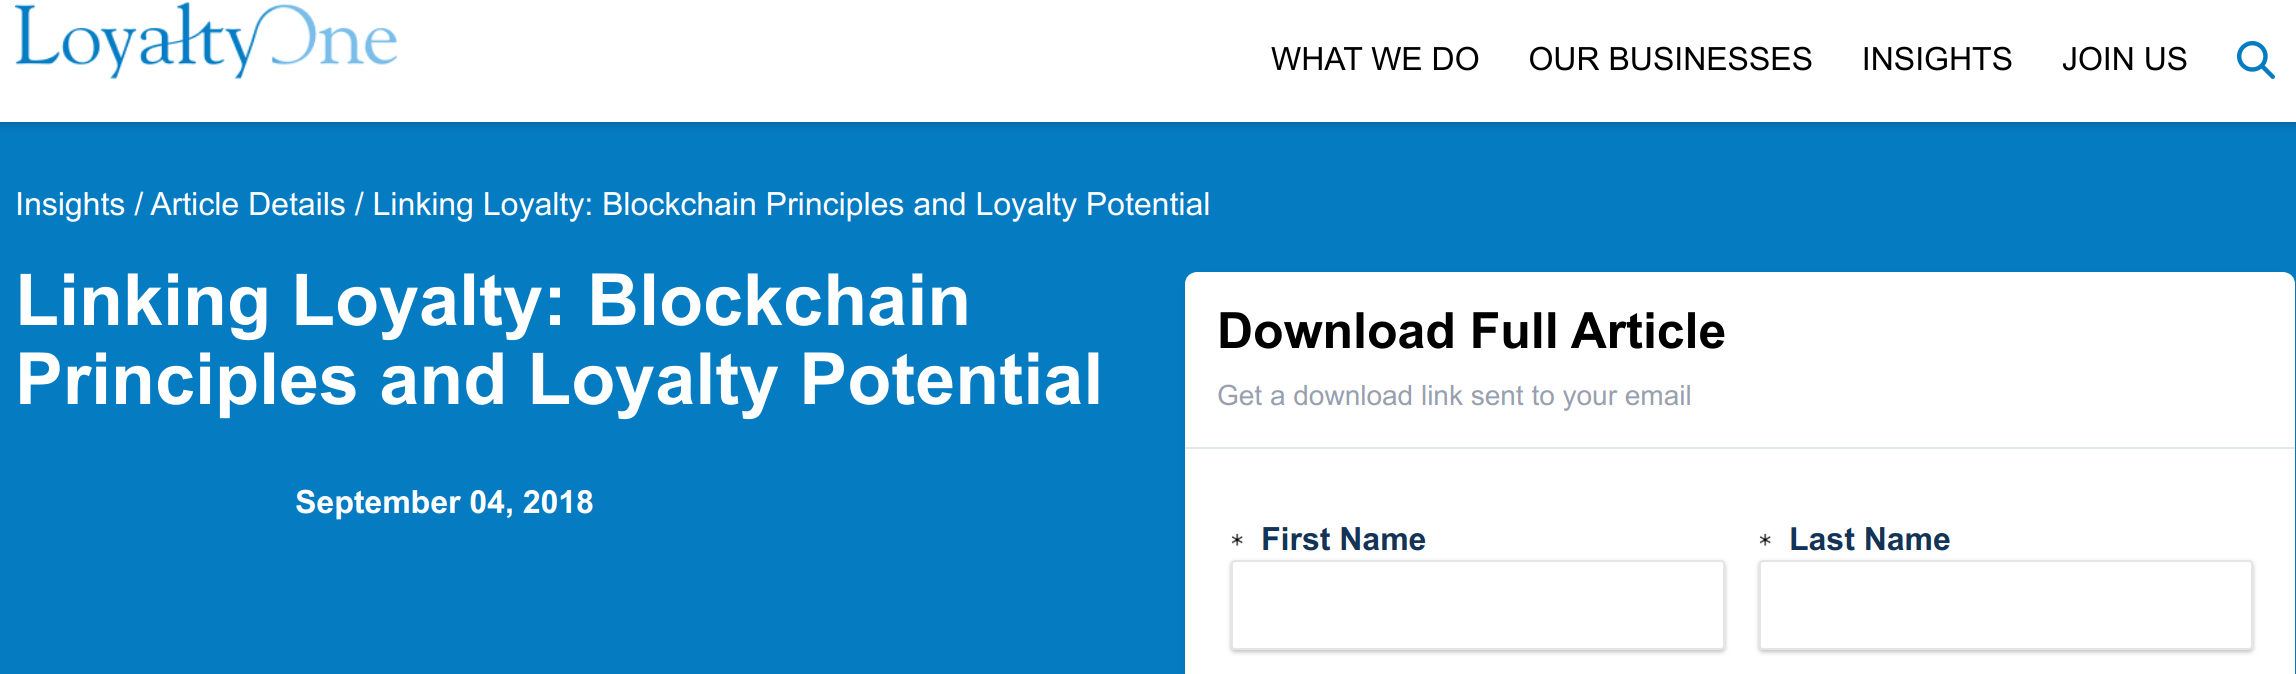
\includegraphics[width=11.5cm]{../pics/loyalty/loyaltyone}
        \caption{\cite{loyaltyone2018:blockchain}}
%        \caption{\url{https://www.loyalty.com/home/insights/article-details/linking-loyalty-blockchain-principles-and-loyalty-potential}}
	\end{figure}
}





\frame{
	\centering\Large{Thank you!}\\
	\vspace{2em}
	{\footnotesize
		Email: \href{mailto:marc@creative-emergy.com}{marc@creative-emergy.com}\\
		Twitter: \href{https://twitter.com/marclijour}{@marclijour}\\
		\href{https://www.creative-emergy.com}{www.creative-emergy.com}
	}
}
\frame{
	\frametitle{References}
	% keyword refers to bib file: references-KEYWORD.bib, and to the Tex file: section-KEYWORD.tex  
	\printbibliography 
}
\end{document}

